%%----------------------------------------------------------------------
\section{Overview}
\label{s:Overview}
%% - - - - - - - - - - - - - - - - - - - - - - - - - - - - - - - - - - -

Project CASSIA (Comprehensive Architecture of Social Simulation for
Inclusive Analysis) aims to develop a framework to administer to
execute large-scale multiagent simulations exhaustively to analyze
socially interactive systems. The framework will realize engineering
environment to design and synthesize social systems like traffics,
economy and politics.

The framework consists of:
\begin{itemize}
  \item
    MASS Planning Module: a manager module conducts effective
    execution plans of simulations among massive possible conditions
    according to available computer resources.
  \item
    MASS Parallel Middleware: an execution middleware provides
    functionality to realize distributed multi-agent simulation on
    many-core computers.
\end{itemize}

%%++++++++++++++++++++++++++++++++++++++++++++++++++++++++++++++++++++++
\begin{figure}
  \centering
  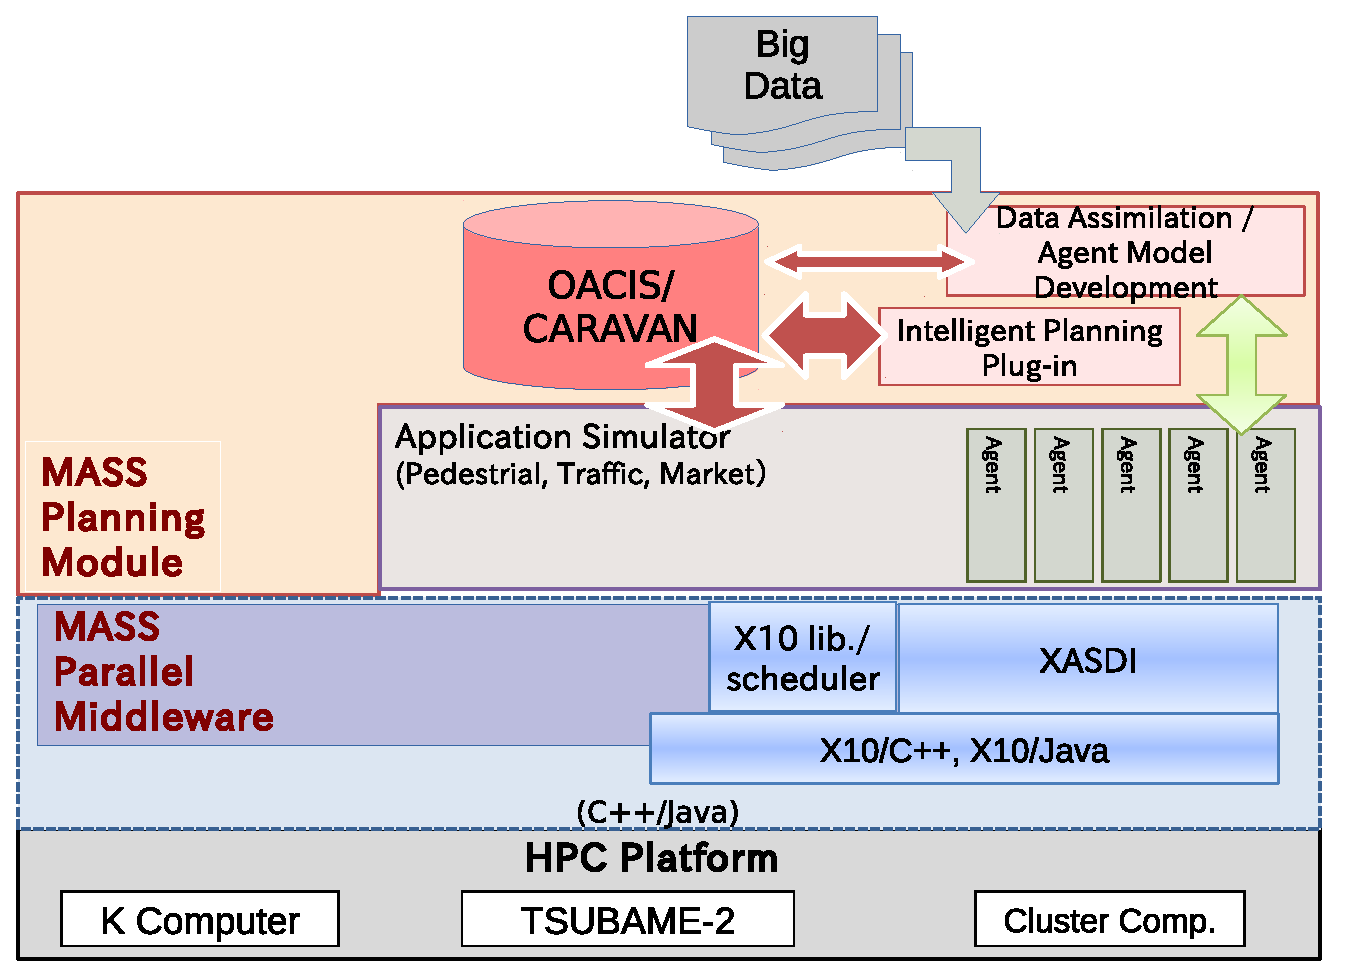
\includegraphics[width=.8\linewidth]{Figs.noda/figure-01.framework.eps}
  \caption{Cassia Framework}
  \label{fig:Figs.noda/figure-01.framework.eps}
\end{figure}
%%++++++++++++++++++++++++++++++++++++++++++++++++++++++++++++++++++++++

